\documentclass[10pt]{article}
\usepackage[a4paper,margin=1.35cm]{geometry}
\usepackage[T1]{fontenc}
\usepackage[utf8]{inputenc}
\usepackage{helvet}
\renewcommand{\familydefault}{\sfdefault}
\usepackage{graphicx}
\usepackage{xcolor}
\usepackage{array}
\usepackage{booktabs}
\usepackage{caption}
\captionsetup{font=scriptsize,labelfont=bf,skip=2pt}
\pagestyle{empty}
\setlength{\parindent}{0pt}
\setlength{\parskip}{2.2pt}
\newcommand{\head}[1]{\vspace{3pt}{\normalsize\bfseries #1}\vspace{1pt}\par}
\newcommand{\sub}[1]{\textbf{#1}}
\newenvironment{tight}{\begin{list}{\textbullet}{\setlength{\leftmargin}{9pt}\setlength{\itemsep}{0.4pt}\setlength{\parsep}{0pt}\setlength{\topsep}{1pt}\setlength{\labelsep}{4pt}}}{\end{list}}
\renewcommand{\arraystretch}{1.1}
% every number below is written by scripts/report_numbers.py from the files in results/
\newcommand{\HeldRows}{TieOut, declared configuration (plans on the graph; a text reader as witness and pointer) & n/a & n/a & n/a & n/a & n/a & n/a \\
Baseline: hybrid retrieval, same model reads (the text reader, alone) & n/a & n/a & n/a & n/a & n/a & n/a \\
Baseline: dense retrieval, same model reads & n/a & n/a & n/a & n/a & n/a & n/a \\
TieOut, one planner (no second planner, no arbiter) & n/a & n/a & n/a & n/a & n/a & n/a \\
TieOut, one picker (no second picker) & n/a & n/a & n/a & n/a & n/a & n/a \\
TieOut, no arbiter & n/a & n/a & n/a & n/a & n/a & n/a \\
TieOut, empty link store & n/a & n/a & n/a & n/a & n/a & n/a \\
TieOut, no equation solving & n/a & n/a & n/a & n/a & n/a & n/a \\
TieOut, no linking (statement concepts only) & n/a & n/a & n/a & n/a & n/a & n/a \\
TieOut, checks off & n/a & n/a & n/a & n/a & n/a & n/a \\
TieOut, no checks read from the question's words & n/a & n/a & n/a & n/a & n/a & n/a \\}
\newcommand{\TierLine}{n/a}
\newcommand{\CostLine}{n/a}
\newcommand{\RoundTenLine}{Round 10 (35 questions nobody had seen; first run of the design in which the text reader can only point at a graph node): the plans alone 24/35, with the text reader 26/35; VERIFIED 1/1, WITNESSED 7/7, CORROBORATED 10/10, FLAGGED 7/12, ABSTAIN 1/5. A version withdrawn the same night, which served answers the reader had written, scored 27/35.}
\newcommand{\CaseLine}{n/a}
\newcommand{\RoundRows}{round 3 & 25/36 & 36/36 \\
round 4 & 22/34 & 35/35 \\
round 5 & 20/36 & 35/36 \\
round 6 & 17/27 & 30/35 \\
round 7 & 23/36 & 35/36 \\
round 8 & 28/35 & 34/35 \\
round 9 & 27/36 & 31/36 \\
round 10 & 26/35 & 28/35 \\
round 11 & 29/36 & 31/36 \\
held-out & n/a & n/a \\}
\newcommand{\StoreLine}{empty store 30/35, 8.9 calls and 1.6 s per question; with links learned on the earlier rounds 30/35, 8.9 calls and 6.4 s}
\newcommand{\ScaleLine}{8667 questions: 8083 correct, 517 abstained, None silent wrong}
\newcommand{\StrictLine}{n/a}
\newcommand{\McNemarLine}{n/a}
\newcommand{\ScaledLine}{n/a}
\newcommand{\TransferLine}{n/a}
\newcommand{\RoadLine}{n/a}

\begin{document}
\small

{\Large\bfseries TieOut: the knowledge graph is the filing's own arithmetic}\par\vspace{2pt}
{\normalsize Madhvansh Choksi \quad\textbar\quad Genloop tech intern take-home \quad\textbar\quad code: \texttt{github.com/Madhvansh/tieout}}\par\vspace{3pt}

\textbf{The idea.} A 10-K is a spreadsheet whose formulas were erased; its numbers still over-determine each other. TieOut recovers the formulas from the printed numbers alone (no model, no XBRL), down the rows and across the columns, and keeps them as the graph. That structure verifies a number, solves for one printed nowhere, names a row that has no label and finds the total column of a segment table. A language model only compiles the question into a typed plan and picks a printed line among masked candidates; it never sees or writes a number, and none of its choices is trusted alone: two independent models make each one and a third is called only when they differ.\par\vspace{3pt}

\begin{minipage}[t]{0.585\textwidth}
\vspace{0pt}
\head{1. Held-out questions, run once}
30 questions by blind authors who never saw the system, committed before any run, gold re-derived by another blind agent, run once on the frozen code (tag \texttt{frozen-v2}) with one free API key and a laptop CPU. Cells are right/asked; precision and recall are macro averages over questions of the facts each answer rests on.

\vspace{2pt}
{\scriptsize\setlength{\tabcolsep}{2.6pt}
\begin{tabular}{@{}p{5.15cm}rrrrrr@{}}
\toprule
 & single & multi & cross & all & P & R \\
\midrule
\HeldRows
\bottomrule
\end{tabular}}

\vspace{2pt}
{\footnotesize \sub{By tier:} \TierLine. \sub{Cost:} \CostLine. \sub{How the two readers split:} \CaseLine. Scores are computed by script against keys the system did not write; no model judges an answer.}
\end{minipage}\hfill
\begin{minipage}[t]{0.39\textwidth}
\vspace{2pt}
\centering
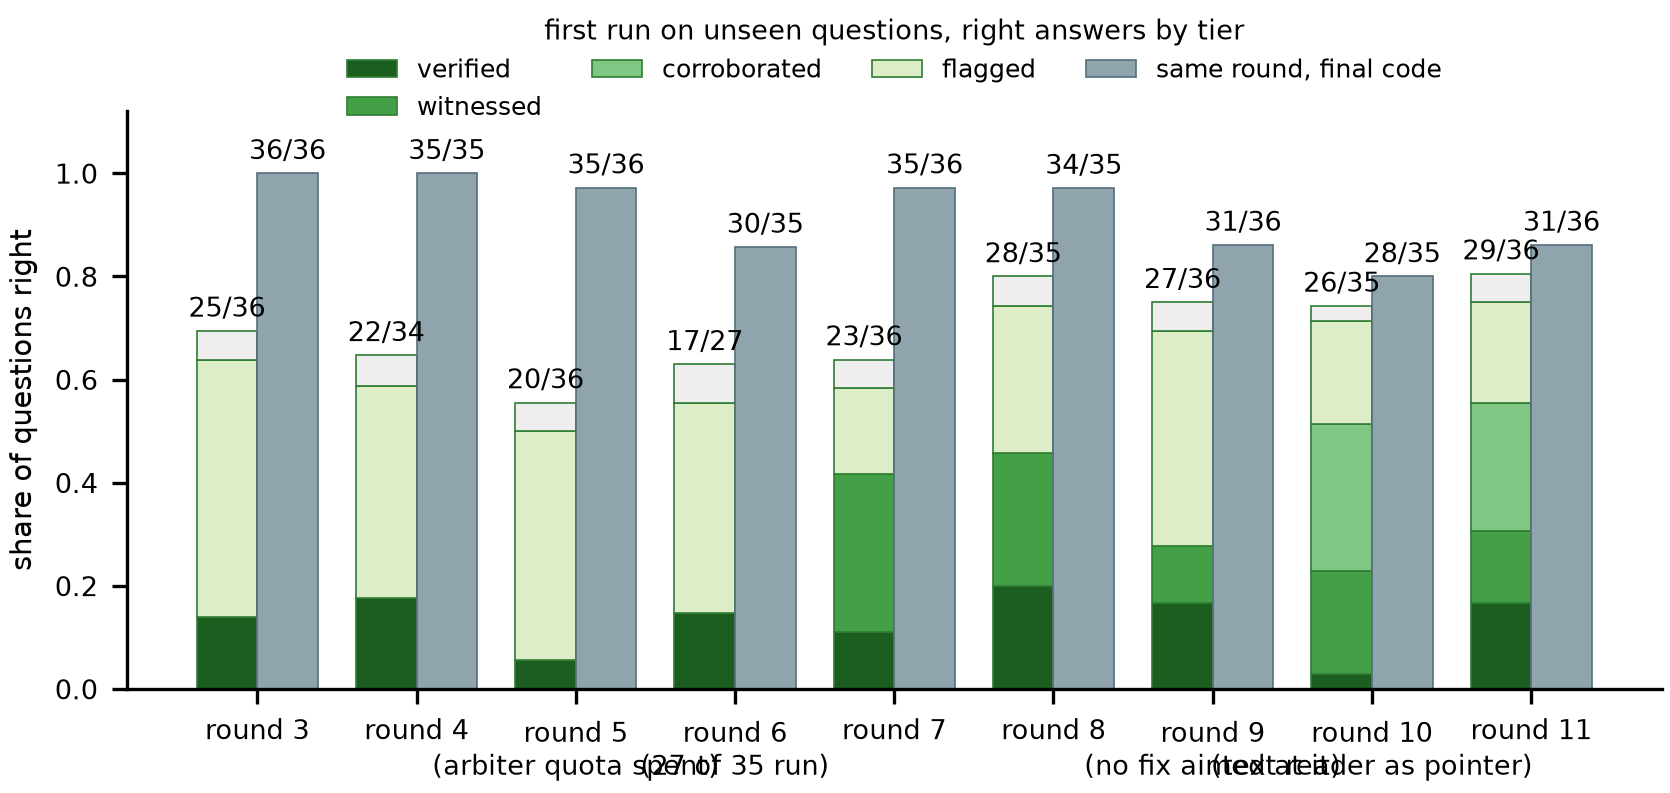
\includegraphics[width=\linewidth]{fig_rounds.png}
\captionof{figure}{Each round of blind questions the first time the system saw it (green, by tier of the right answers) and on the final code (grey). The held-out round was never fixed against.}
\end{minipage}

\head{2. We measured our own overfitting}
The first development set flattered the system: 84 of 87 there, and 25 of 36 on the first batch of questions it had never seen. So the work ran in rounds. Blind authors (agents that read only the PDFs and the list of used questions; a new persona each round: analyst, auditor, credit analyst, journalist, test engineer) write a round; a gate drops near copies of held-out questions without anyone reading them; the system runs once and that number is recorded; only then are the misses fixed, by class, with general rules, never a rule about one company. First-run accuracy stayed 15 to 30 points below the same day's development numbers. Part of that is adaptation; part may be that fresh questions are different (Recht et al.\ 2019 saw the same drop with no reuse at all), so we report both and do not call the gap overfitting alone. What the rounds taught, one class each: the total column is the one that sums the others; a year printed once over three columns; a fourth quarter of any line as year minus nine months; a quarterly header that spans two columns; one company's segment against another's (\texttt{compare}); a figure dated by the date printed beside it in a sentence; a count stated with a scale in its row label; a table cut where a row carries a footnote marker; an equal value that is a coincidence, not a tie.

\head{3. The graph learns}
A link from a phrase to a printed line is kept only when the answer it led to matched its gold, and only then reused. On the last fresh round, same code and same questions: \StoreLine.

\newpage
\head{4. Method}
\begin{tight}
\item \emph{Tables} from word coordinates: columns from the right edges of numbers, periods from header dates, scale from captions and row labels, rows kept whole across footnote markers.
\item \emph{Equations.} A row is a subtotal only if a signed run of rows above it sums to it in every period; a column is the total only if it sums the columns beside it. Checks: SUM, TIE (a value printed twice), RATIO (income over shares pins the scale), CARRY (last year's column equals last year's filing).
\item \emph{Names.} 47 concepts kept as data; a label proposes, structure confirms. Every other table row and every numeric sentence is a node, linked to a phrase the first time a question needs it.
\item \emph{Solve.} A number printed nowhere comes from the one equation where it is the only unknown (a fourth quarter, an identity).
\item \emph{Plan.} A model writes a typed plan (get, calc, compare, rank, filter, members ...); a deterministic executor returns the answer with proof leaves (filing, page, printed text).
\item \emph{Four eyes.} Two readers plan each question: a free hosted model and a 4B model fine-tuned on Kaggle on paraphrased questions, run on the laptop. Plans are compared on what they compute. Two pickers choose each printed line, compared on the figure the pick yields. A strong free model (about 20 calls a day) arbitrates only disagreements.
\item \emph{Tiers.} VERIFIED: every number inside a passing equation, no line chosen by a model. WITNESSED: the numbers tie out and two models chose the same line. FLAGGED: answered, weakness named. ABSTAIN: says what is missing.
\end{tight}

\head{5. Where it fails, by class}
{\scriptsize
\begin{tabular}{@{}p{3.1cm}p{14.4cm}@{}}
\toprule
Class & What happens, with one page each \\
\midrule
\FailRows
\bottomrule
\end{tabular}}

\head{6. Evidence from keys we did not write}
{\scriptsize
\begin{tabular}{@{}p{5.6cm}p{11.9cm}@{}}
\toprule
\EvidenceRows
\bottomrule
\end{tabular}}

\head{7. What did not work}
\begin{tight}
\item Tuning on one development set (above). Trusting one model's plan or pick: the cheap model slips on about one plan in eight.
\item Distant supervision of a row picker by equal values: of 1,790 training pairs 805 were coincidences; the picker trained on them was not used.
\item A link kept for ever: one bad pick failed every later question that used its phrase. Links are now outcome-gated.
\item Planners fine-tuned on template questions: 84 to 88\% on synthetic phrasings, far lower on real ones. Paraphrase training lifted the 4B model from 137 to 152 of 194 development questions.
\item A model judge to admit a binding (it threw away half the right ones); hosted Gemma (503s); a strong model as the only planner (20 calls a day).
\end{tight}

\head{8. AI use}
Claude Code (several sessions and sub-agents, coordinated through shared logs) wrote all the code and ran every experiment; blind agents wrote and re-derived the benchmark. I set the direction and made the rulings (README, ``How I used AI''), twice against the AI's own plan.
\end{document}
